\section{Zadanie 5} 
Pora wyznaczyć regulator dla naszego niestabilnego obiektu. Użyjemy struktury drugiego modelu w przestrzeni stanu. Ogólna struktura regulatora to:
\[
 u(k)=-KX(k)
\]

Wektor $K$ obliczamy poleceniem \mintinline{matlab}{Kd = acker(Ad,Bd,[z1 z2 z3])}, gdzie za \mintinline{matlab}{z1}, \mintinline{matlab}{z2} i \mintinline{matlab}{z3} ustalamy bieguny układu zamkniętego.
\begin{figure}[H]
\centering
 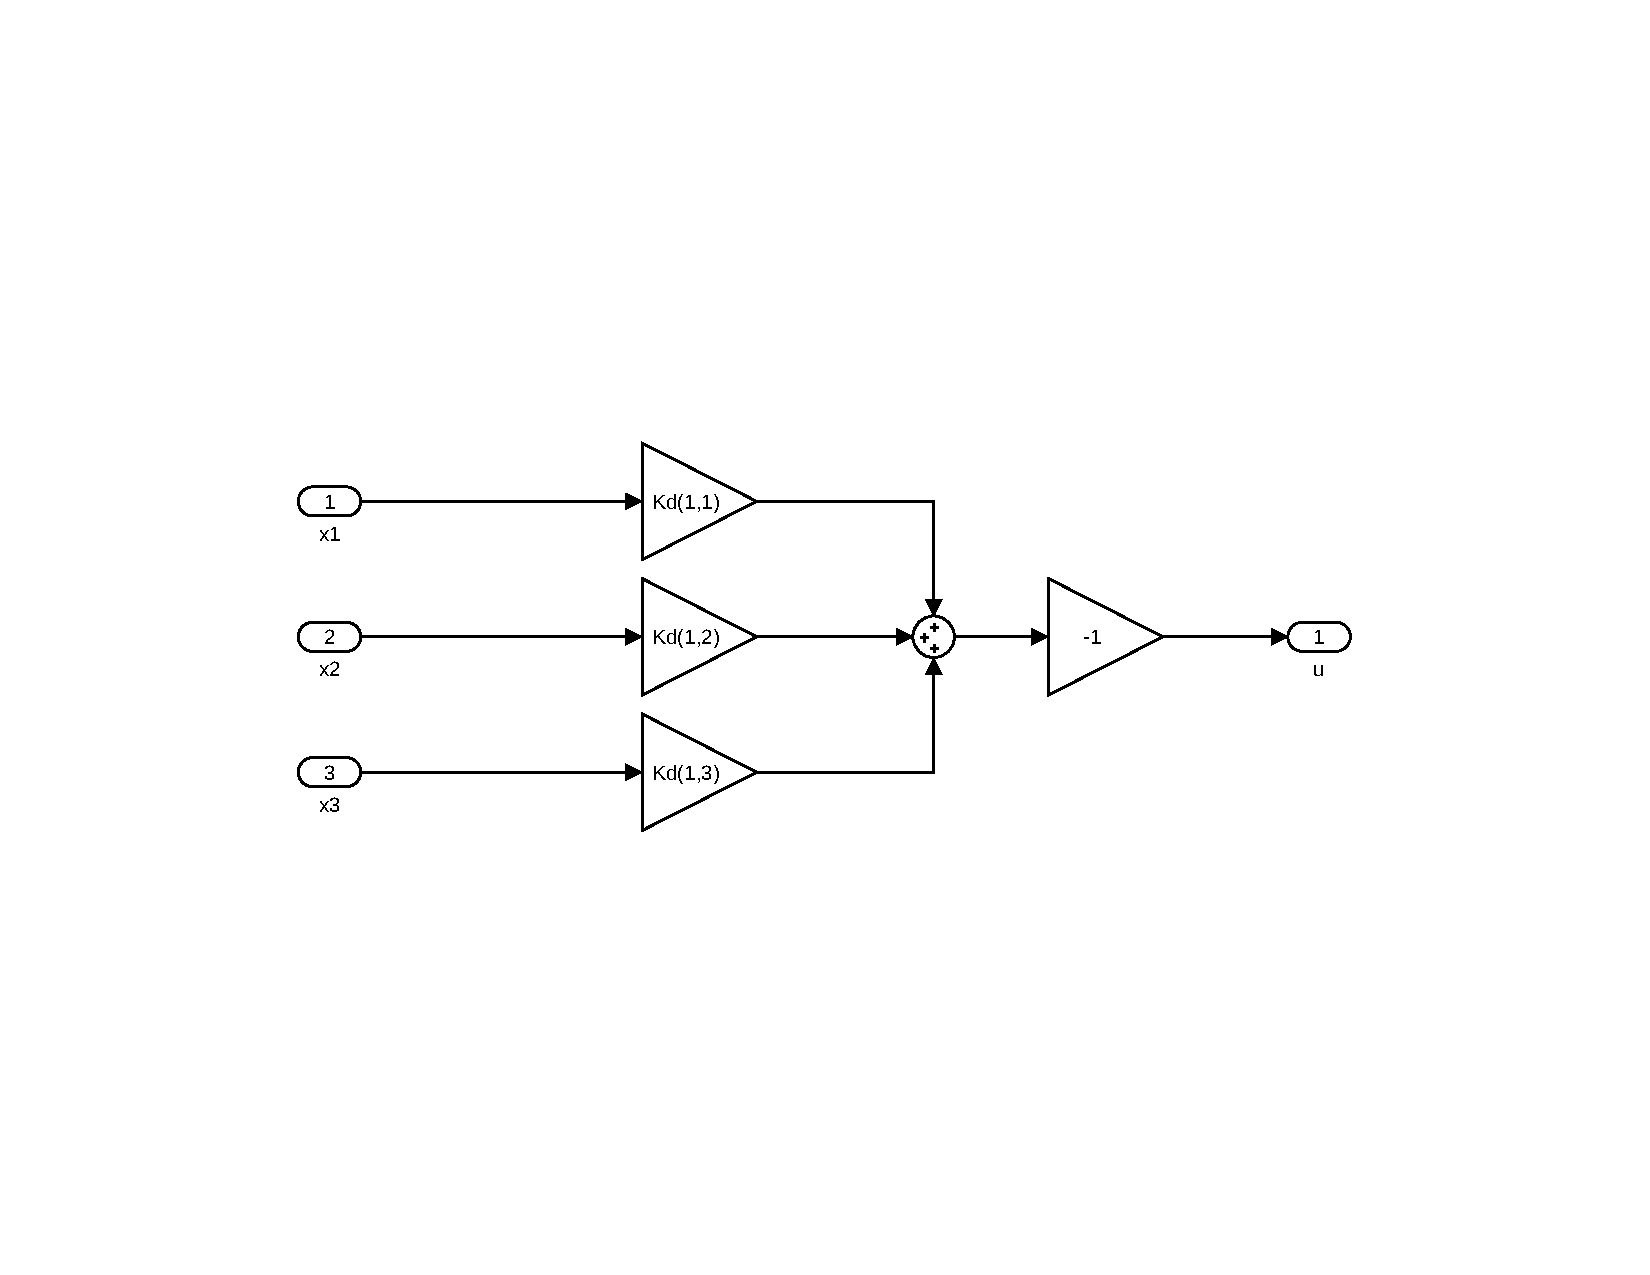
\includegraphics[width=\textwidth]{img/reg.pdf}
\caption{Struktura regulatora.}
\end{figure}

\begin{figure}[H]
\centering
 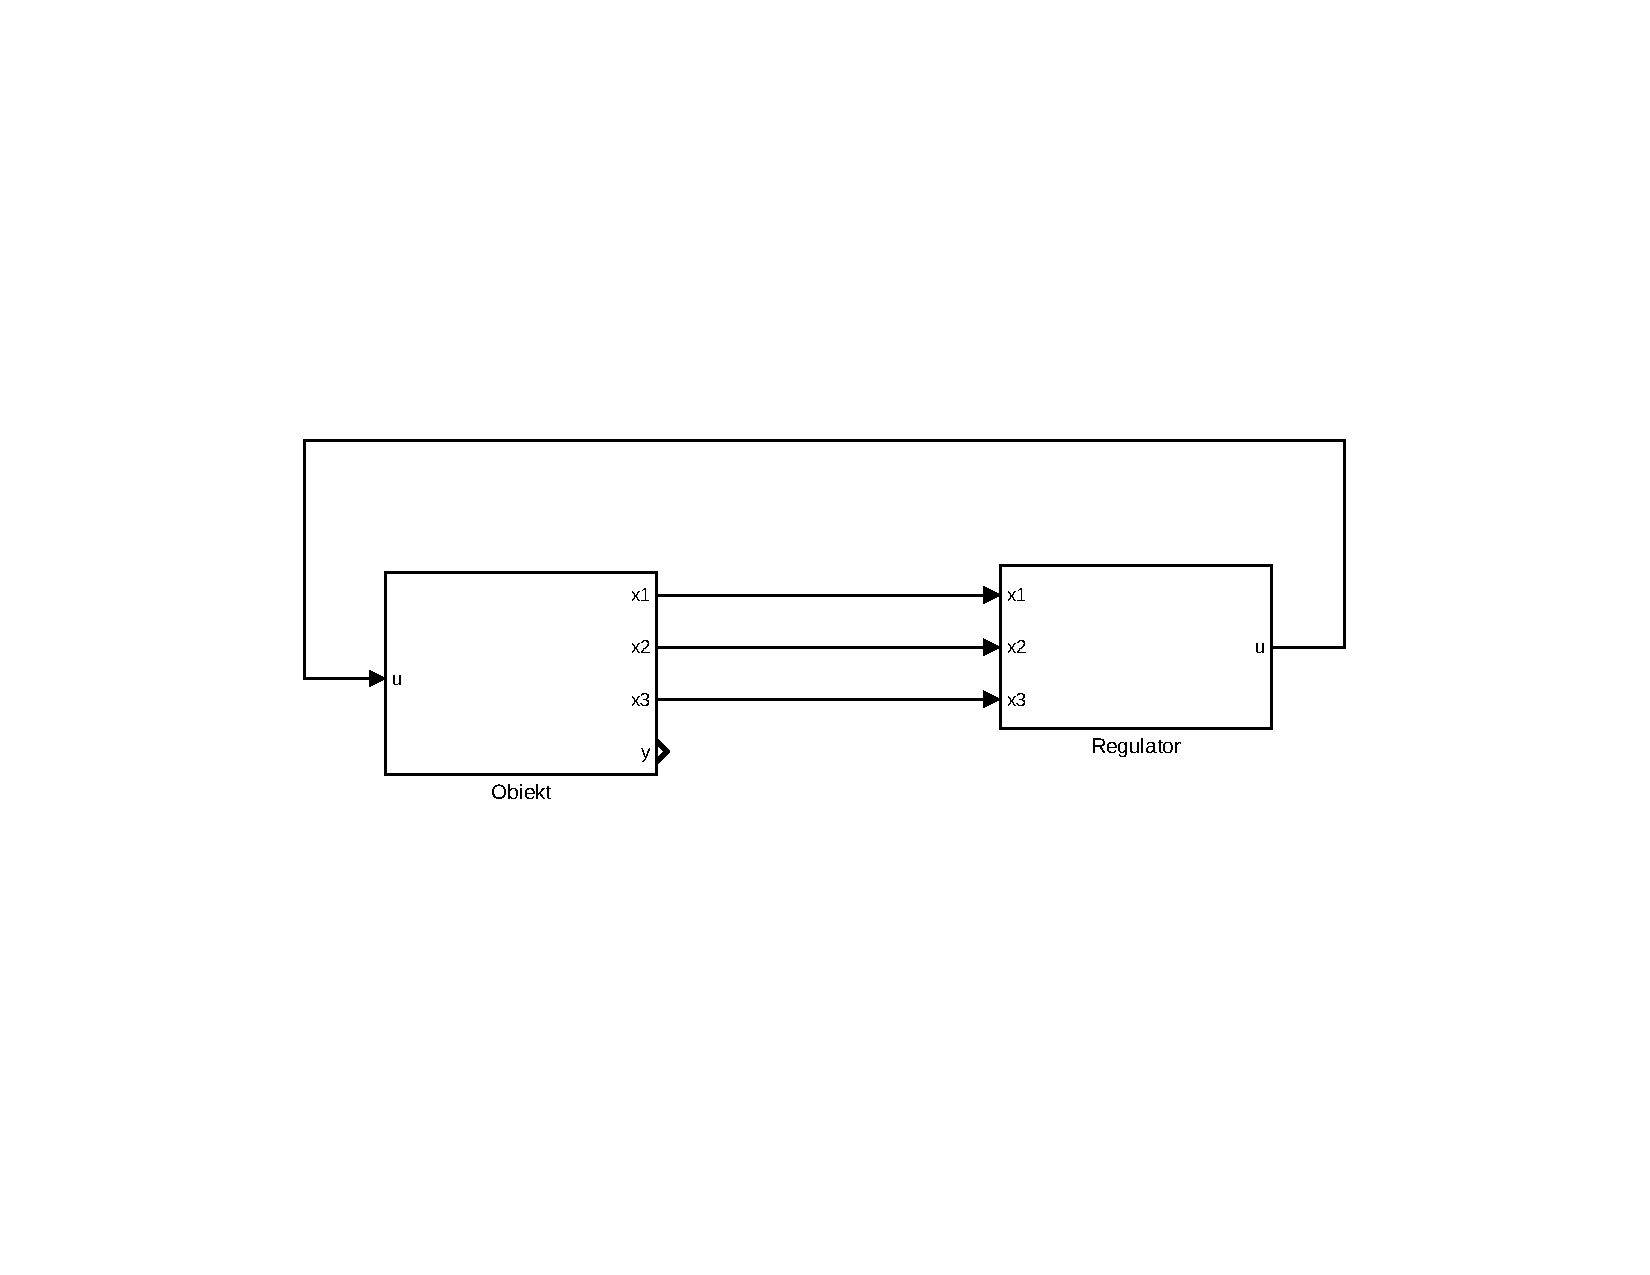
\includegraphics[width=\textwidth]{img/objreg.pdf}
\caption{Struktura układu zamkniętego.}
\end{figure}

\subsection{Trzy takie same bieguny}

W zależności od odległości biegunów od środka układu współrzędnych, regulator szybko, wolno, lub w ogóle sprowadza układ do stanu ustalonego.

\begin{figure}[H]
\centering
 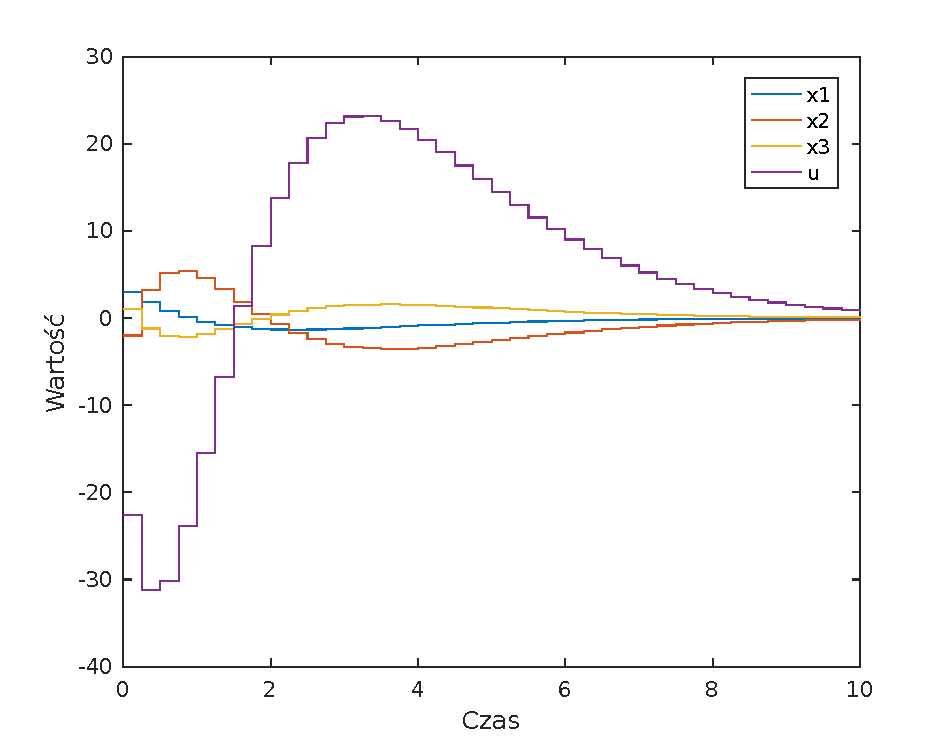
\includegraphics[width=\textwidth]{img/plot1.pdf}
\caption{Wartości stanu dla trzech biegunów $z_{b1} = z_{b2} = z_{b3} = 0,8$.}
\end{figure}

\subsection{Dwa bieguny dominujące}
Dwa bieguny powinny być szybkie, a zatem jak najbliżej środka układu współrzędnych.
Można ustalić $z_{b2} = z_{b3} = 0,1$, oraz $z_{b1} = 0,6$.
To daje nam przebieg taki, jak na wykresie.
\begin{figure}[H]
\centering
 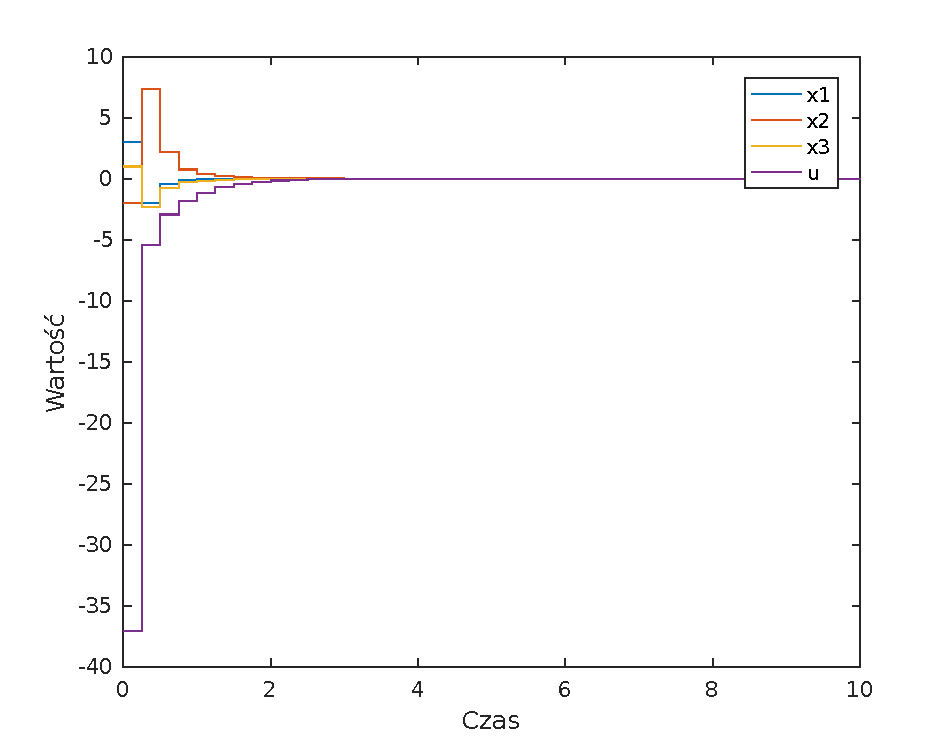
\includegraphics[width=\textwidth]{img/plot2.pdf}
\caption{Wartości stanu dla dwóch biegunów dominujących.}
\end{figure}
Takie ustawienie biegunów pozwala na łatwe manipulowanie dominującym biegunem, aby dobrać akceptowalne wartości sterowania.

\subsection{Inne bieguny}

\begin{figure}[H]
\centering
 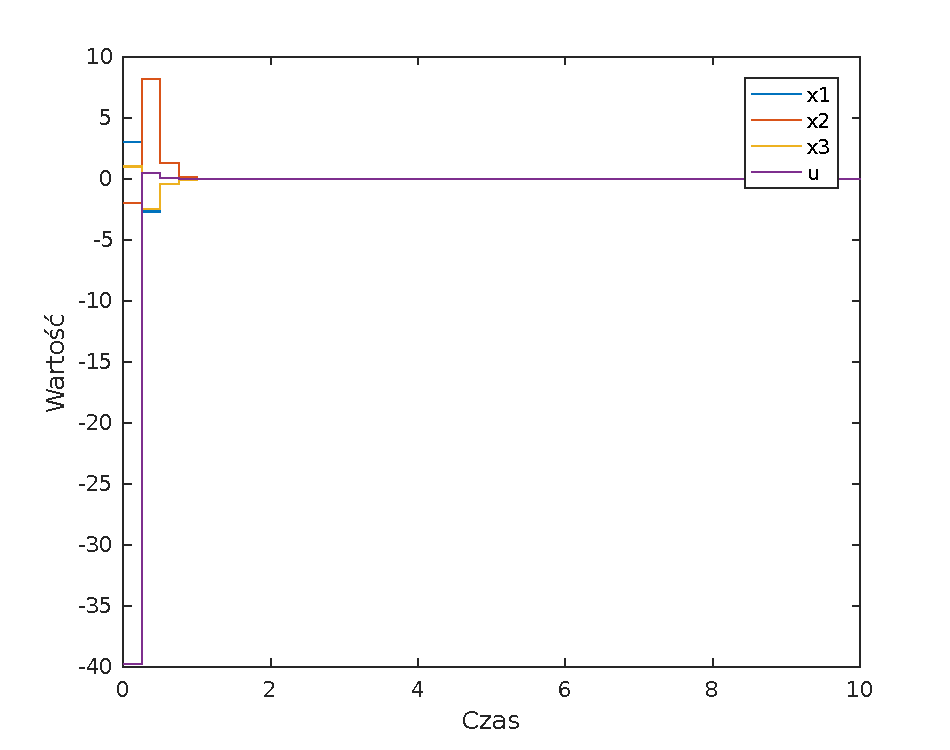
\includegraphics[width=\textwidth]{img/plot3.pdf}
\caption{Regulator $z_{b1}=0$, $z_{b2}=0,2$ i $z_{b3}=0,3$.}
\end{figure}

\begin{figure}[H]
\centering
 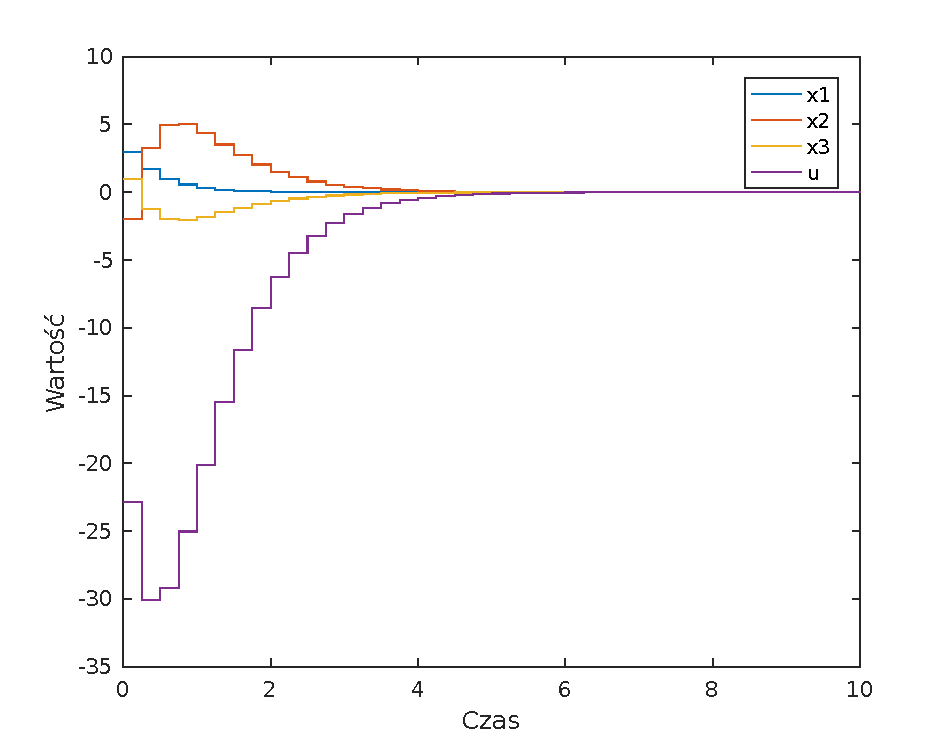
\includegraphics[width=\textwidth]{img/plot4.pdf}
\caption{Regulator $z_{b1}=0,2$, $z_{b2}=0,4$ i $z_{b3}=0,2$.}
\end{figure}

\begin{figure}[H]
\centering
 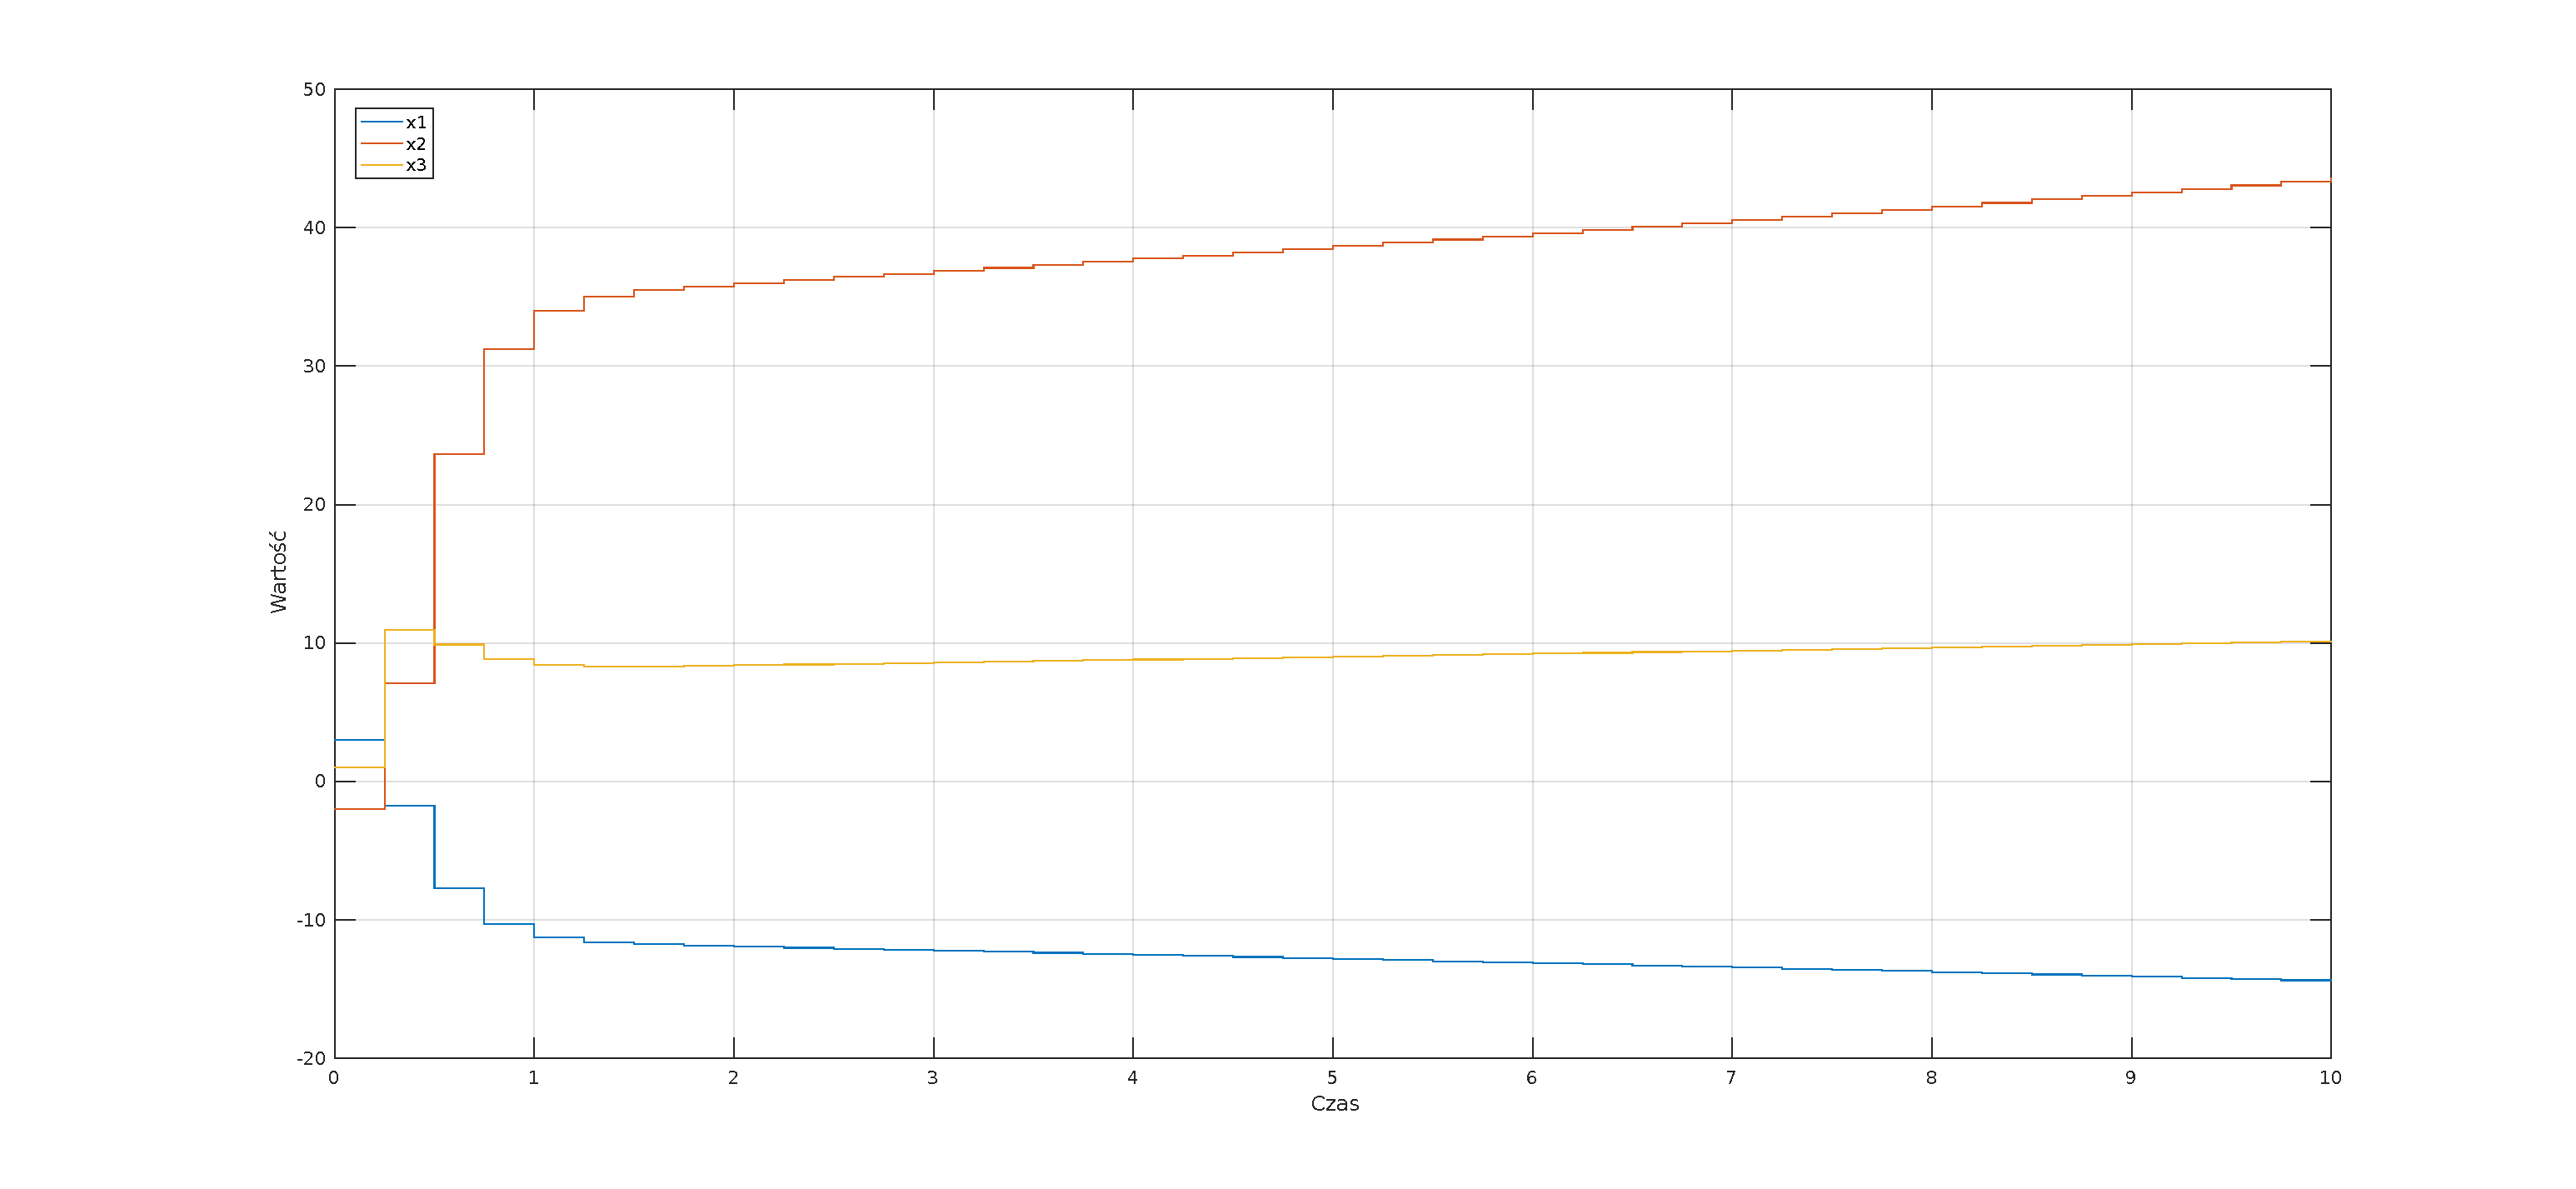
\includegraphics[width=\textwidth]{img/plot5.pdf}
\caption{Regulator $z_{b1}=0,6$, $z_{b2}=0,2$ i $z_{b3}=0,5$.}
\end{figure}

\begin{figure}[H]
\centering
 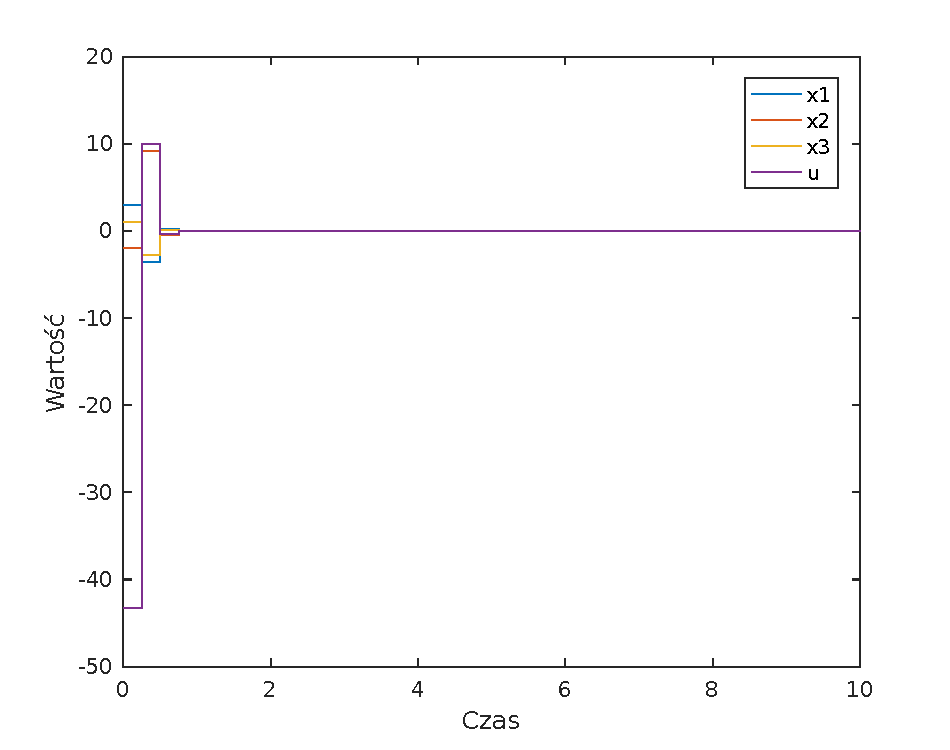
\includegraphics[width=\textwidth]{img/plot6.pdf}
\caption{Regulator $z_{b1}=z_{b2}=z_{b3}=0$.}
\end{figure}

Najlepsze znalezione ustawienie posiada bieguny $z_{b1}=0,3$, $z_{b2}=0,3$ i $z_{b3}=0,7$.
Nie obciąża zbytnio układu wykonawczego, a przede wszystkim nie zmienia kierunku jego działania.
Jednocześnie wartości stanu zbiegają do zera w ciągu kilku sekund.

\begin{figure}[H]
\centering
 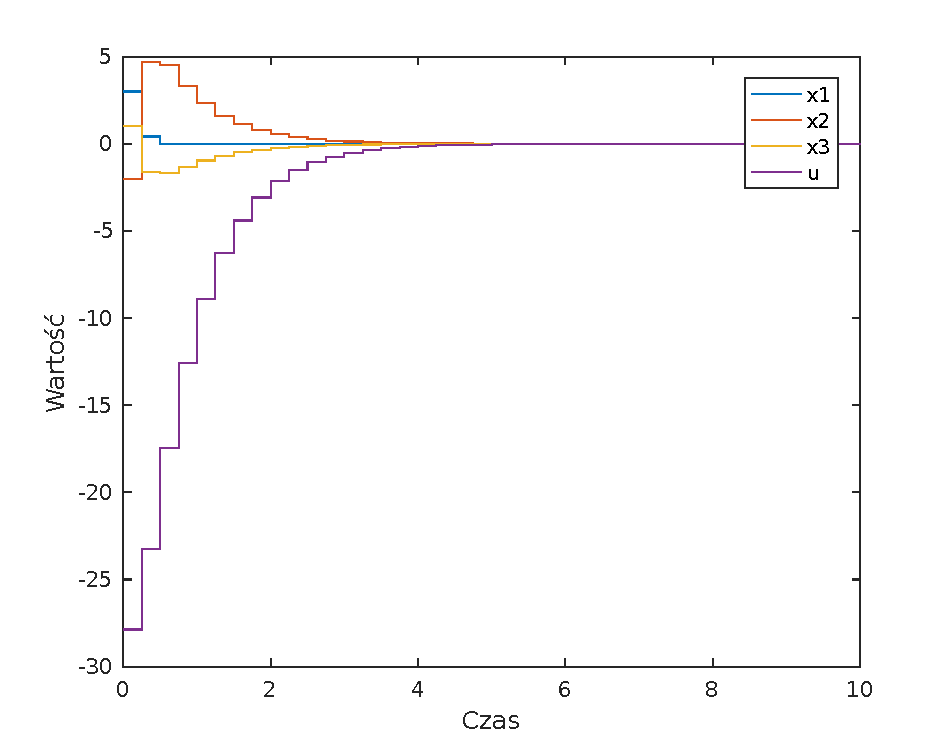
\includegraphics[width=\textwidth]{img/plot7.pdf}
\caption{Regulator $z_{b1}=0,3$, $z_{b2}=0,3$ i $z_{b3}=0,7$.}
\end{figure}



